\documentclass[twoside]{book}

% Packages required by doxygen
\usepackage{fixltx2e}
\usepackage{calc}
\usepackage{doxygen}
\usepackage[export]{adjustbox} % also loads graphicx
\usepackage{graphicx}
\usepackage[utf8]{inputenc}
\usepackage{makeidx}
\usepackage{multicol}
\usepackage{multirow}
\PassOptionsToPackage{warn}{textcomp}
\usepackage{textcomp}
\usepackage[nointegrals]{wasysym}
\usepackage[table]{xcolor}

% Font selection
\usepackage[T1]{fontenc}
\usepackage[scaled=.90]{helvet}
\usepackage{courier}
\usepackage{amssymb}
\usepackage{sectsty}
\renewcommand{\familydefault}{\sfdefault}
\allsectionsfont{%
  \fontseries{bc}\selectfont%
  \color{darkgray}%
}
\renewcommand{\DoxyLabelFont}{%
  \fontseries{bc}\selectfont%
  \color{darkgray}%
}
\newcommand{\+}{\discretionary{\mbox{\scriptsize$\hookleftarrow$}}{}{}}

% Page & text layout
\usepackage{geometry}
\geometry{%
  a4paper,%
  top=2.5cm,%
  bottom=2.5cm,%
  left=2.5cm,%
  right=2.5cm%
}
\tolerance=750
\hfuzz=15pt
\hbadness=750
\setlength{\emergencystretch}{15pt}
\setlength{\parindent}{0cm}
\setlength{\parskip}{3ex plus 2ex minus 2ex}
\makeatletter
\renewcommand{\paragraph}{%
  \@startsection{paragraph}{4}{0ex}{-1.0ex}{1.0ex}{%
    \normalfont\normalsize\bfseries\SS@parafont%
  }%
}
\renewcommand{\subparagraph}{%
  \@startsection{subparagraph}{5}{0ex}{-1.0ex}{1.0ex}{%
    \normalfont\normalsize\bfseries\SS@subparafont%
  }%
}
\makeatother

% Headers & footers
\usepackage{fancyhdr}
\pagestyle{fancyplain}
\fancyhead[LE]{\fancyplain{}{\bfseries\thepage}}
\fancyhead[CE]{\fancyplain{}{}}
\fancyhead[RE]{\fancyplain{}{\bfseries\leftmark}}
\fancyhead[LO]{\fancyplain{}{\bfseries\rightmark}}
\fancyhead[CO]{\fancyplain{}{}}
\fancyhead[RO]{\fancyplain{}{\bfseries\thepage}}
\fancyfoot[LE]{\fancyplain{}{}}
\fancyfoot[CE]{\fancyplain{}{}}
\fancyfoot[RE]{\fancyplain{}{\bfseries\scriptsize Generated by Doxygen }}
\fancyfoot[LO]{\fancyplain{}{\bfseries\scriptsize Generated by Doxygen }}
\fancyfoot[CO]{\fancyplain{}{}}
\fancyfoot[RO]{\fancyplain{}{}}
\renewcommand{\footrulewidth}{0.4pt}
\renewcommand{\chaptermark}[1]{%
  \markboth{#1}{}%
}
\renewcommand{\sectionmark}[1]{%
  \markright{\thesection\ #1}%
}

% Indices & bibliography
\usepackage{natbib}
\usepackage[titles]{tocloft}
\setcounter{tocdepth}{3}
\setcounter{secnumdepth}{5}
\makeindex

% Hyperlinks (required, but should be loaded last)
\usepackage{ifpdf}
\ifpdf
  \usepackage[pdftex,pagebackref=true]{hyperref}
\else
  \usepackage[ps2pdf,pagebackref=true]{hyperref}
\fi
\hypersetup{%
  colorlinks=true,%
  linkcolor=blue,%
  citecolor=blue,%
  unicode%
}

% Custom commands
\newcommand{\clearemptydoublepage}{%
  \newpage{\pagestyle{empty}\cleardoublepage}%
}

\usepackage{caption}
\captionsetup{labelsep=space,justification=centering,font={bf},singlelinecheck=off,skip=4pt,position=top}

%===== C O N T E N T S =====

\begin{document}

% Titlepage & ToC
\hypersetup{pageanchor=false,
             bookmarksnumbered=true,
             pdfencoding=unicode
            }
\pagenumbering{roman}
\begin{titlepage}
\vspace*{7cm}
\begin{center}%
{\Large Simple 7bit A\+S\+C\+II Encoding/\+Decoding library }\\
\vspace*{1cm}
{\large Generated by Doxygen 1.8.11}\\
\end{center}
\end{titlepage}
\clearemptydoublepage
\tableofcontents
\clearemptydoublepage
\pagenumbering{arabic}
\hypersetup{pageanchor=true}

%--- Begin generated contents ---
\chapter{Encoding scheme}
\label{index}\hypertarget{index}{}The encode function accept 8-\/bit A\+S\+C\+II characters, and compress the string by removing the most significant bit and packing such 7-\/bit characters in the 8-\/bit bytes, so that all the bits are used (each 8 character sequence would then fit in 7 bytes)

For example, consider the following string and it\textquotesingle{}s hexadecimal representation\+:


\begin{DoxyCode}
1 ASCII string: H    e    l    l    o   
2   Hex values: 0x48 0x65 0x6C 0x6C 0x6F    
\end{DoxyCode}


We can represent all the chars in 8bit binary form, and also in 7bit form removing the most significant bit\+:


\begin{DoxyCode}
1 8bit form: 01001000 01100101 01101100 01101100 01101111
2 7bit form: .1001000 .1100101 .1101100 .1101100 .1101111
\end{DoxyCode}


Now we move the L\+SB bit from the 2nd byte to the M\+SB bit of the 1st byte\+:


\begin{DoxyCode}
1                           *
2 Move bit: .1001000 .110010. .1101100 .1101100 .1101111
3 Move bit: 11001000 .110010. .1101100 .1101100 .1101111
4           *
\end{DoxyCode}


We can shift the 2nd byte by one space, the one free\+:


\begin{DoxyCode}
1                  ------>
2 Shift: 11001000 .110010. .1101100 .1101100 .1101111
3 Shift: 11001000 ..110010 .1101100 .1101100 .1101111
\end{DoxyCode}


And we can repeat the first step, taking this time 2 L\+SB bits from the 3rd character\+:


\begin{DoxyCode}
1                                    **
2 Move bits: 11001000 ..110010 .11011.. .1101100 .1101111
3 Move bits: 11001000 00110010 .1101100 .1101100 .1101111
4                     **
\end{DoxyCode}


And repeat this process for every character, obtaining\+:


\begin{DoxyCode}
1     Result: 11001000 00110010 10011011 11111101 00000110
2 Hex values: 0xC8     0x32     0x9B     0xFD     0x06
\end{DoxyCode}
 
\chapter{File Index}
\section{File List}
Here is a list of all files with brief descriptions\+:\begin{DoxyCompactList}
\item\contentsline{section}{\hyperlink{encdec_8c}{encdec.\+c} }{\pageref{encdec_8c}}{}
\item\contentsline{section}{\hyperlink{encdec_8h}{encdec.\+h} }{\pageref{encdec_8h}}{}
\item\contentsline{section}{\hyperlink{main_8c}{main.\+c} \\*Testing app for the 7bit encoder/decoder library }{\pageref{main_8c}}{}
\end{DoxyCompactList}

\chapter{File Documentation}
\hypertarget{encdec_8c}{}\section{encdec.\+c File Reference}
\label{encdec_8c}\index{encdec.\+c@{encdec.\+c}}
{\ttfamily \#include $<$stdio.\+h$>$}\\*
{\ttfamily \#include $<$stdlib.\+h$>$}\\*
{\ttfamily \#include $<$string.\+h$>$}\\*
{\ttfamily \#include $<$stddef.\+h$>$}\\*
{\ttfamily \#include $<$stdint.\+h$>$}\\*
{\ttfamily \#include $<$stdbool.\+h$>$}\\*
{\ttfamily \#include \char`\"{}encdec.\+h\char`\"{}}\\*
Include dependency graph for encdec.\+c\+:
\nopagebreak
\begin{figure}[H]
\begin{center}
\leavevmode
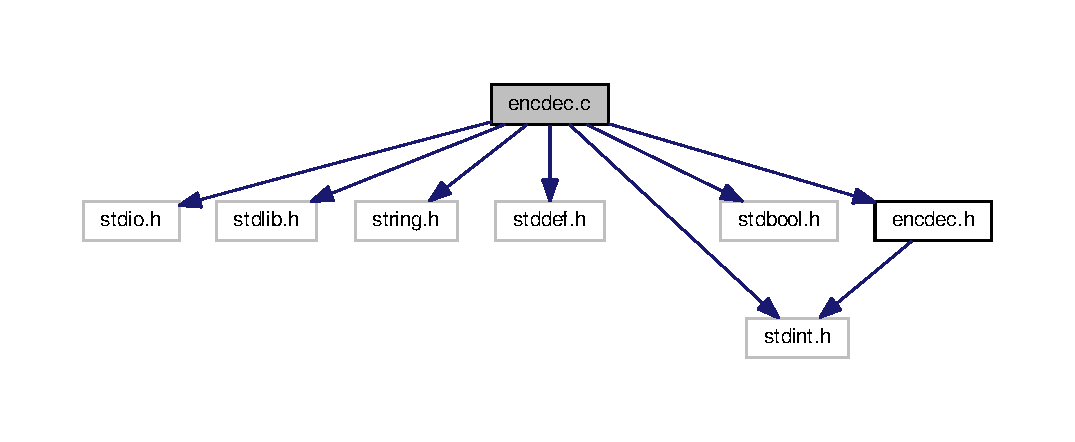
\includegraphics[width=350pt]{encdec_8c__incl}
\end{center}
\end{figure}
\subsection*{Macros}
\begin{DoxyCompactItemize}
\item 
\#define \hyperlink{encdec_8c_a8f8ffe1f5e961bcf9f4373d868c923d5}{B\+I\+T\+M\+A\+S\+K\+\_\+7\+B\+I\+TS}~0x7F
\end{DoxyCompactItemize}
\subsection*{Functions}
\begin{DoxyCompactItemize}
\item 
int32\+\_\+t \hyperlink{encdec_8c_a1ed55e9e612c6f9dde8c7cdc90d19769}{text\+\_\+7bit\+\_\+encode} (const char $\ast$txt\+\_\+in, char $\ast$txt\+\_\+out)
\begin{DoxyCompactList}\small\item\em Encode an A\+S\+C\+II string into a 7 bit compressed representation. \end{DoxyCompactList}\item 
int32\+\_\+t \hyperlink{encdec_8c_ad7af7323d34249a7dc0636b5eb0b2e7a}{text\+\_\+7bit\+\_\+decode} (const char $\ast$txt\+\_\+in, char $\ast$txt\+\_\+out)
\begin{DoxyCompactList}\small\item\em Decode a 7 bit compressed representation into a string. \end{DoxyCompactList}\end{DoxyCompactItemize}


\subsection{Macro Definition Documentation}
\index{encdec.\+c@{encdec.\+c}!B\+I\+T\+M\+A\+S\+K\+\_\+7\+B\+I\+TS@{B\+I\+T\+M\+A\+S\+K\+\_\+7\+B\+I\+TS}}
\index{B\+I\+T\+M\+A\+S\+K\+\_\+7\+B\+I\+TS@{B\+I\+T\+M\+A\+S\+K\+\_\+7\+B\+I\+TS}!encdec.\+c@{encdec.\+c}}
\subsubsection[{\texorpdfstring{B\+I\+T\+M\+A\+S\+K\+\_\+7\+B\+I\+TS}{BITMASK_7BITS}}]{\setlength{\rightskip}{0pt plus 5cm}\#define B\+I\+T\+M\+A\+S\+K\+\_\+7\+B\+I\+TS~0x7F}\hypertarget{encdec_8c_a8f8ffe1f5e961bcf9f4373d868c923d5}{}\label{encdec_8c_a8f8ffe1f5e961bcf9f4373d868c923d5}


Definition at line 9 of file encdec.\+c.



\subsection{Function Documentation}
\index{encdec.\+c@{encdec.\+c}!text\+\_\+7bit\+\_\+decode@{text\+\_\+7bit\+\_\+decode}}
\index{text\+\_\+7bit\+\_\+decode@{text\+\_\+7bit\+\_\+decode}!encdec.\+c@{encdec.\+c}}
\subsubsection[{\texorpdfstring{text\+\_\+7bit\+\_\+decode(const char $\ast$txt\+\_\+in, char $\ast$txt\+\_\+out)}{text_7bit_decode(const char *txt_in, char *txt_out)}}]{\setlength{\rightskip}{0pt plus 5cm}int32\+\_\+t text\+\_\+7bit\+\_\+decode (
\begin{DoxyParamCaption}
\item[{const char $\ast$}]{txt\+\_\+in, }
\item[{char $\ast$}]{txt\+\_\+out}
\end{DoxyParamCaption}
)}\hypertarget{encdec_8c_ad7af7323d34249a7dc0636b5eb0b2e7a}{}\label{encdec_8c_ad7af7323d34249a7dc0636b5eb0b2e7a}


Decode a 7 bit compressed representation into a string. 


\begin{DoxyParams}[1]{Parameters}
\mbox{\tt in}  & {\em txt\+\_\+in} & Null-\/terminated 7-\/bit encoded string \\
\hline
\mbox{\tt out}  & {\em txt\+\_\+out} & Null-\/terminated decoded A\+S\+C\+II string \\
\hline
\end{DoxyParams}
\begin{DoxyReturn}{Returns}
size of the output data ($>$0) or error ($<$0) 
\end{DoxyReturn}


Definition at line 75 of file encdec.\+c.

\index{encdec.\+c@{encdec.\+c}!text\+\_\+7bit\+\_\+encode@{text\+\_\+7bit\+\_\+encode}}
\index{text\+\_\+7bit\+\_\+encode@{text\+\_\+7bit\+\_\+encode}!encdec.\+c@{encdec.\+c}}
\subsubsection[{\texorpdfstring{text\+\_\+7bit\+\_\+encode(const char $\ast$txt\+\_\+in, char $\ast$txt\+\_\+out)}{text_7bit_encode(const char *txt_in, char *txt_out)}}]{\setlength{\rightskip}{0pt plus 5cm}int32\+\_\+t text\+\_\+7bit\+\_\+encode (
\begin{DoxyParamCaption}
\item[{const char $\ast$}]{txt\+\_\+in, }
\item[{char $\ast$}]{txt\+\_\+out}
\end{DoxyParamCaption}
)}\hypertarget{encdec_8c_a1ed55e9e612c6f9dde8c7cdc90d19769}{}\label{encdec_8c_a1ed55e9e612c6f9dde8c7cdc90d19769}


Encode an A\+S\+C\+II string into a 7 bit compressed representation. 


\begin{DoxyParams}[1]{Parameters}
\mbox{\tt in}  & {\em txt\+\_\+in} & Null-\/terminated A\+S\+C\+II string to encode \\
\hline
\mbox{\tt out}  & {\em txt\+\_\+out} & 7-\/bit encoded string, null terminated \\
\hline
\end{DoxyParams}
\begin{DoxyReturn}{Returns}
size of the output data or error ($<$0) 
\end{DoxyReturn}


Definition at line 18 of file encdec.\+c.


\hypertarget{encdec_8h}{}\section{encdec.\+h File Reference}
\label{encdec_8h}\index{encdec.\+h@{encdec.\+h}}
{\ttfamily \#include $<$stdint.\+h$>$}\\*
Include dependency graph for encdec.\+h\+:
\nopagebreak
\begin{figure}[H]
\begin{center}
\leavevmode
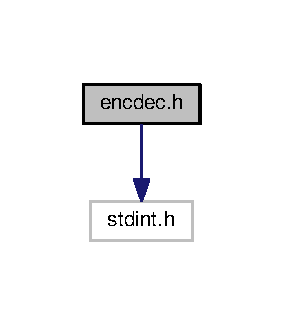
\includegraphics[width=136pt]{encdec_8h__incl}
\end{center}
\end{figure}
This graph shows which files directly or indirectly include this file\+:
\nopagebreak
\begin{figure}[H]
\begin{center}
\leavevmode
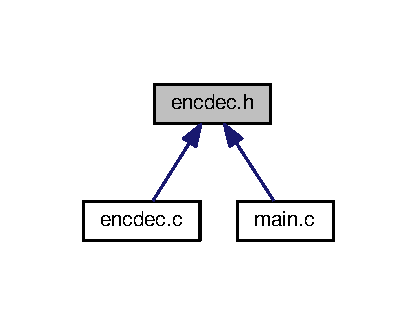
\includegraphics[width=200pt]{encdec_8h__dep__incl}
\end{center}
\end{figure}
\subsection*{Macros}
\begin{DoxyCompactItemize}
\item 
\#define \hyperlink{encdec_8h_adba6e73bc444514871898203133c02cc}{L\+I\+B\+\_\+\+E\+R\+R\+\_\+\+N\+U\+L\+L\+\_\+\+P\+TR}~-\/1
\item 
\#define \hyperlink{encdec_8h_a3e39be0f446773fef1c51f2588d6108a}{L\+I\+B\+\_\+\+E\+R\+R\+\_\+\+N\+O\+N\+\_\+\+A\+S\+C\+II}~-\/2
\end{DoxyCompactItemize}
\subsection*{Functions}
\begin{DoxyCompactItemize}
\item 
int32\+\_\+t \hyperlink{encdec_8h_a1ed55e9e612c6f9dde8c7cdc90d19769}{text\+\_\+7bit\+\_\+encode} (const char $\ast$txt\+\_\+in, char $\ast$txt\+\_\+out)
\begin{DoxyCompactList}\small\item\em Encode an A\+S\+C\+II string into a 7 bit compressed representation. \end{DoxyCompactList}\item 
int32\+\_\+t \hyperlink{encdec_8h_ad7af7323d34249a7dc0636b5eb0b2e7a}{text\+\_\+7bit\+\_\+decode} (const char $\ast$txt\+\_\+in, char $\ast$txt\+\_\+out)
\begin{DoxyCompactList}\small\item\em Decode a 7 bit compressed representation into a string. \end{DoxyCompactList}\end{DoxyCompactItemize}


\subsection{Macro Definition Documentation}
\index{encdec.\+h@{encdec.\+h}!L\+I\+B\+\_\+\+E\+R\+R\+\_\+\+N\+O\+N\+\_\+\+A\+S\+C\+II@{L\+I\+B\+\_\+\+E\+R\+R\+\_\+\+N\+O\+N\+\_\+\+A\+S\+C\+II}}
\index{L\+I\+B\+\_\+\+E\+R\+R\+\_\+\+N\+O\+N\+\_\+\+A\+S\+C\+II@{L\+I\+B\+\_\+\+E\+R\+R\+\_\+\+N\+O\+N\+\_\+\+A\+S\+C\+II}!encdec.\+h@{encdec.\+h}}
\subsubsection[{\texorpdfstring{L\+I\+B\+\_\+\+E\+R\+R\+\_\+\+N\+O\+N\+\_\+\+A\+S\+C\+II}{LIB_ERR_NON_ASCII}}]{\setlength{\rightskip}{0pt plus 5cm}\#define L\+I\+B\+\_\+\+E\+R\+R\+\_\+\+N\+O\+N\+\_\+\+A\+S\+C\+II~-\/2}\hypertarget{encdec_8h_a3e39be0f446773fef1c51f2588d6108a}{}\label{encdec_8h_a3e39be0f446773fef1c51f2588d6108a}


Definition at line 4 of file encdec.\+h.

\index{encdec.\+h@{encdec.\+h}!L\+I\+B\+\_\+\+E\+R\+R\+\_\+\+N\+U\+L\+L\+\_\+\+P\+TR@{L\+I\+B\+\_\+\+E\+R\+R\+\_\+\+N\+U\+L\+L\+\_\+\+P\+TR}}
\index{L\+I\+B\+\_\+\+E\+R\+R\+\_\+\+N\+U\+L\+L\+\_\+\+P\+TR@{L\+I\+B\+\_\+\+E\+R\+R\+\_\+\+N\+U\+L\+L\+\_\+\+P\+TR}!encdec.\+h@{encdec.\+h}}
\subsubsection[{\texorpdfstring{L\+I\+B\+\_\+\+E\+R\+R\+\_\+\+N\+U\+L\+L\+\_\+\+P\+TR}{LIB_ERR_NULL_PTR}}]{\setlength{\rightskip}{0pt plus 5cm}\#define L\+I\+B\+\_\+\+E\+R\+R\+\_\+\+N\+U\+L\+L\+\_\+\+P\+TR~-\/1}\hypertarget{encdec_8h_adba6e73bc444514871898203133c02cc}{}\label{encdec_8h_adba6e73bc444514871898203133c02cc}


Definition at line 3 of file encdec.\+h.



\subsection{Function Documentation}
\index{encdec.\+h@{encdec.\+h}!text\+\_\+7bit\+\_\+decode@{text\+\_\+7bit\+\_\+decode}}
\index{text\+\_\+7bit\+\_\+decode@{text\+\_\+7bit\+\_\+decode}!encdec.\+h@{encdec.\+h}}
\subsubsection[{\texorpdfstring{text\+\_\+7bit\+\_\+decode(const char $\ast$txt\+\_\+in, char $\ast$txt\+\_\+out)}{text_7bit_decode(const char *txt_in, char *txt_out)}}]{\setlength{\rightskip}{0pt plus 5cm}int32\+\_\+t text\+\_\+7bit\+\_\+decode (
\begin{DoxyParamCaption}
\item[{const char $\ast$}]{txt\+\_\+in, }
\item[{char $\ast$}]{txt\+\_\+out}
\end{DoxyParamCaption}
)}\hypertarget{encdec_8h_ad7af7323d34249a7dc0636b5eb0b2e7a}{}\label{encdec_8h_ad7af7323d34249a7dc0636b5eb0b2e7a}


Decode a 7 bit compressed representation into a string. 


\begin{DoxyParams}[1]{Parameters}
\mbox{\tt in}  & {\em txt\+\_\+in} & Null-\/terminated 7-\/bit encoded string \\
\hline
\mbox{\tt out}  & {\em txt\+\_\+out} & Null-\/terminated decoded A\+S\+C\+II string \\
\hline
\end{DoxyParams}
\begin{DoxyReturn}{Returns}
size of the output data ($>$0) or error\+\_\+code ($<$0)
\end{DoxyReturn}

\begin{DoxyParams}[1]{Parameters}
\mbox{\tt in}  & {\em txt\+\_\+in} & Null-\/terminated 7-\/bit encoded string \\
\hline
\mbox{\tt out}  & {\em txt\+\_\+out} & Null-\/terminated decoded A\+S\+C\+II string \\
\hline
\end{DoxyParams}
\begin{DoxyReturn}{Returns}
size of the output data ($>$0) or error ($<$0) 
\end{DoxyReturn}


Definition at line 75 of file encdec.\+c.

\index{encdec.\+h@{encdec.\+h}!text\+\_\+7bit\+\_\+encode@{text\+\_\+7bit\+\_\+encode}}
\index{text\+\_\+7bit\+\_\+encode@{text\+\_\+7bit\+\_\+encode}!encdec.\+h@{encdec.\+h}}
\subsubsection[{\texorpdfstring{text\+\_\+7bit\+\_\+encode(const char $\ast$txt\+\_\+in, char $\ast$txt\+\_\+out)}{text_7bit_encode(const char *txt_in, char *txt_out)}}]{\setlength{\rightskip}{0pt plus 5cm}int32\+\_\+t text\+\_\+7bit\+\_\+encode (
\begin{DoxyParamCaption}
\item[{const char $\ast$}]{txt\+\_\+in, }
\item[{char $\ast$}]{txt\+\_\+out}
\end{DoxyParamCaption}
)}\hypertarget{encdec_8h_a1ed55e9e612c6f9dde8c7cdc90d19769}{}\label{encdec_8h_a1ed55e9e612c6f9dde8c7cdc90d19769}


Encode an A\+S\+C\+II string into a 7 bit compressed representation. 


\begin{DoxyParams}[1]{Parameters}
\mbox{\tt in}  & {\em txt\+\_\+in} & Null-\/terminated A\+S\+C\+II string to encode \\
\hline
\mbox{\tt out}  & {\em txt\+\_\+out} & 7-\/bit encoded string, null terminated \\
\hline
\end{DoxyParams}
\begin{DoxyReturn}{Returns}
size of the output data or error\+\_\+code ($<$0)
\end{DoxyReturn}

\begin{DoxyParams}[1]{Parameters}
\mbox{\tt in}  & {\em txt\+\_\+in} & Null-\/terminated A\+S\+C\+II string to encode \\
\hline
\mbox{\tt out}  & {\em txt\+\_\+out} & 7-\/bit encoded string, null terminated \\
\hline
\end{DoxyParams}
\begin{DoxyReturn}{Returns}
size of the output data or error ($<$0) 
\end{DoxyReturn}


Definition at line 18 of file encdec.\+c.


\hypertarget{_l_i_b_8md}{}\section{L\+I\+B.\+md File Reference}
\label{_l_i_b_8md}\index{L\+I\+B.\+md@{L\+I\+B.\+md}}

\hypertarget{main_8c}{}\section{main.\+c File Reference}
\label{main_8c}\index{main.\+c@{main.\+c}}


Testing app for the 7bit encoder/decoder library.  


{\ttfamily \#include $<$stdint.\+h$>$}\\*
{\ttfamily \#include $<$assert.\+h$>$}\\*
{\ttfamily \#include $<$stdlib.\+h$>$}\\*
{\ttfamily \#include $<$stdio.\+h$>$}\\*
{\ttfamily \#include $<$string.\+h$>$}\\*
{\ttfamily \#include \char`\"{}aenc/encdec.\+h\char`\"{}}\\*
Include dependency graph for main.\+c\+:
\nopagebreak
\begin{figure}[H]
\begin{center}
\leavevmode
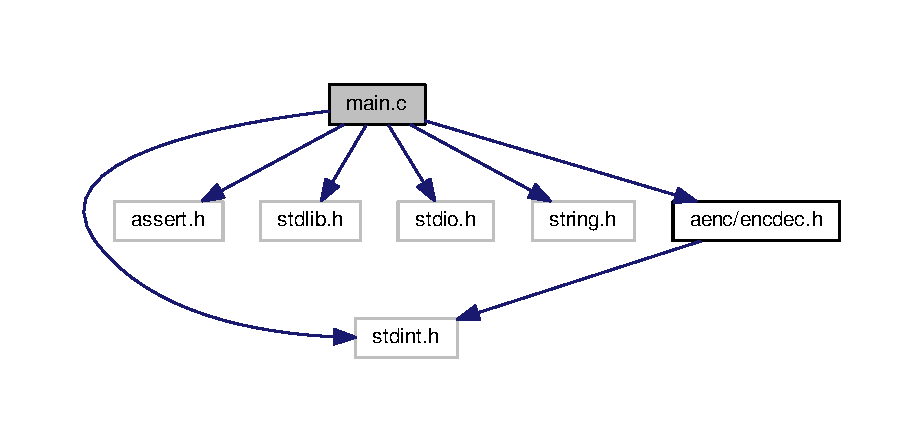
\includegraphics[width=350pt]{main_8c__incl}
\end{center}
\end{figure}
\subsection*{Macros}
\begin{DoxyCompactItemize}
\item 
\#define \hyperlink{main_8c_ab5187269936538ffb8ccbbe7115ffdbc}{M\+A\+X\+\_\+\+S\+T\+R\+I\+NG}~128
\end{DoxyCompactItemize}
\subsection*{Functions}
\begin{DoxyCompactItemize}
\item 
void \hyperlink{main_8c_ac2517d3824ac044ff5c083a01672996b}{print\+\_\+string} (char $\ast$txt)
\item 
int \hyperlink{main_8c_a840291bc02cba5474a4cb46a9b9566fe}{main} (void)
\begin{DoxyCompactList}\small\item\em Example application to test the library. \end{DoxyCompactList}\end{DoxyCompactItemize}


\subsection{Detailed Description}
Testing app for the 7bit encoder/decoder library. 

\begin{DoxyAuthor}{Author}
Enrico D\textquotesingle{}Abramo
\end{DoxyAuthor}
\begin{DoxyDate}{Date}
3/24/2020 
\end{DoxyDate}


\subsection{Macro Definition Documentation}
\index{main.\+c@{main.\+c}!M\+A\+X\+\_\+\+S\+T\+R\+I\+NG@{M\+A\+X\+\_\+\+S\+T\+R\+I\+NG}}
\index{M\+A\+X\+\_\+\+S\+T\+R\+I\+NG@{M\+A\+X\+\_\+\+S\+T\+R\+I\+NG}!main.\+c@{main.\+c}}
\subsubsection[{\texorpdfstring{M\+A\+X\+\_\+\+S\+T\+R\+I\+NG}{MAX_STRING}}]{\setlength{\rightskip}{0pt plus 5cm}\#define M\+A\+X\+\_\+\+S\+T\+R\+I\+NG~128}\hypertarget{main_8c_ab5187269936538ffb8ccbbe7115ffdbc}{}\label{main_8c_ab5187269936538ffb8ccbbe7115ffdbc}


Definition at line 16 of file main.\+c.



\subsection{Function Documentation}
\index{main.\+c@{main.\+c}!main@{main}}
\index{main@{main}!main.\+c@{main.\+c}}
\subsubsection[{\texorpdfstring{main(void)}{main(void)}}]{\setlength{\rightskip}{0pt plus 5cm}int main (
\begin{DoxyParamCaption}
\item[{void}]{}
\end{DoxyParamCaption}
)}\hypertarget{main_8c_a840291bc02cba5474a4cb46a9b9566fe}{}\label{main_8c_a840291bc02cba5474a4cb46a9b9566fe}


Example application to test the library. 



Definition at line 45 of file main.\+c.

\index{main.\+c@{main.\+c}!print\+\_\+string@{print\+\_\+string}}
\index{print\+\_\+string@{print\+\_\+string}!main.\+c@{main.\+c}}
\subsubsection[{\texorpdfstring{print\+\_\+string(char $\ast$txt)}{print_string(char *txt)}}]{\setlength{\rightskip}{0pt plus 5cm}void print\+\_\+string (
\begin{DoxyParamCaption}
\item[{char $\ast$}]{txt}
\end{DoxyParamCaption}
)}\hypertarget{main_8c_ac2517d3824ac044ff5c083a01672996b}{}\label{main_8c_ac2517d3824ac044ff5c083a01672996b}


Definition at line 18 of file main.\+c.


%--- End generated contents ---

% Index
\backmatter
\newpage
\phantomsection
\clearemptydoublepage
\addcontentsline{toc}{chapter}{Index}
\printindex

\end{document}
